\documentclass[12pt]{article}
\usepackage[utf8]{inputenc}
\newcommand\preamble{
    \usepackage[italian]{babel}
    \usepackage{geometry}
    \usepackage{amsmath}
    \usepackage{amssymb}
    \usepackage{graphicx}
    \usepackage{ulem}
    \usepackage[dvipsnames]{xcolor}

    \geometry{margin=2cm}
    \let\olditemize\itemize
    \renewcommand\itemize{\olditemize\setlength\itemsep{0em}}
    \graphicspath{{../Immagini/}}

    \author{Lorenzo Vaccarecci}
}
\preamble

\title{Gestore delle strutture di memorizzazione - Buffer}
\date{15 Marzo 2024}

\begin{document}
\maketitle
\section{Introduzione}
L'obiettivo è minimizzare il numero di accessi alla memoria non volatile, che è molto lenta. Il buffer viene gestito dal DBMS.\\
Mantenere più blocchi possibili in memoria principale in modo da evitare riletture da memoria non volatile.
\section{Il Buffer}
Il buffer è organizzato in pagine, che hanno la stessa dimensione delle pagine/blocchi su disco.
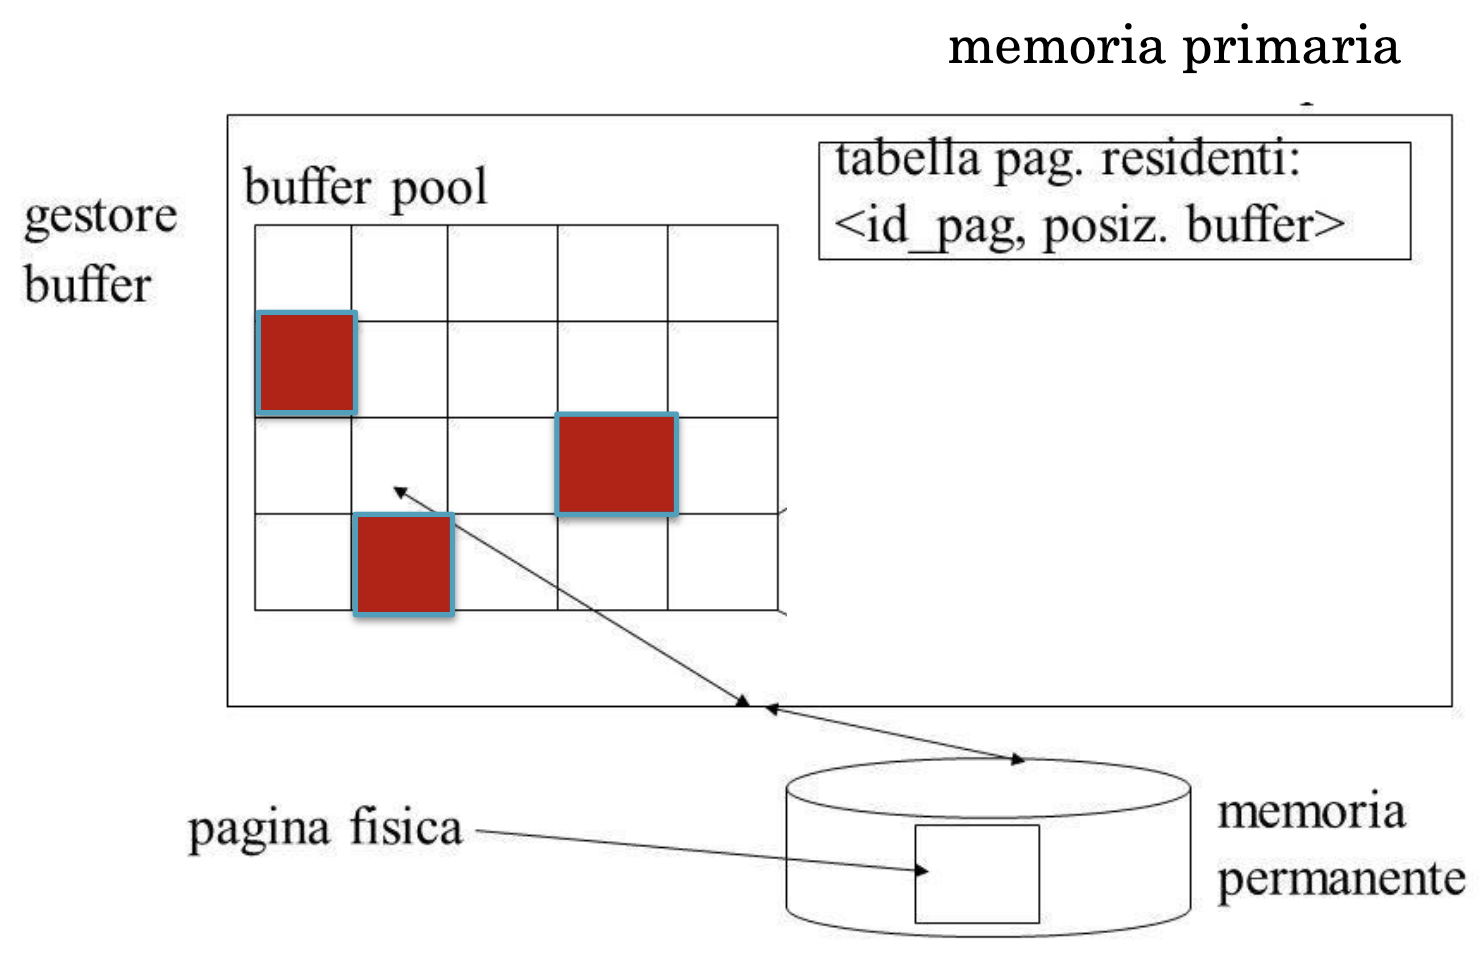
\includegraphics[width=\textwidth]{buffer.png}
\section{Gestione del buffer}
Dopo l'esecuzione di una interrogazione, il \textbf{Buffer Manager} (BM) controlla prima nel buffer e se la pagina non è presente:
\begin{itemize}
    \item Cerca una pagina nel buffer libera
    \item Se non è presente, cerca una pagina da sostituire
    \item Se la pagina da sostituire è stata modificata, la scrive su disco
    \item A questo punto la pagina è libera e può essere sovrascritta
\end{itemize}
Quando una pagina è presente nel buffer, le operazioni di lettura e scrittura possono essere effettuate su di essa.
\subsection{Politiche di sostituzione}
Il BM sceglie quale politica usare in base alle informazioni che ha.
\begin{description}
    \item[\textbf{LRU (Least Recently Used)}]: La pagina meno recentemente usata viene sostituita. 
    \item[\textbf{MRU (Most Recently Used)}]: La pagina più recentemente usata viene sostituita. Spesso viene usata questa politica perchè il sistema sa che dovrà rileggere questo blocco ma non nell'immediato futuro.
\end{description}
\end{document}